\chapter{2013年“三项工作”汇报}
\section{2013年度工程投资、物资采购、宣传促销执行情况} \sanhao

\indent 三联公司2013年工程投资、物资采购、宣传促销年度
计划36个项目,共计15204.56万元\footnote{由川渝中烟物资中心统一采购的丝束和成型纸等未纳入统计}。
实际执行 34个项目,共计8588.4万元,其中公开招标19项,涉及金额 5505.75万元,占比64.1\%。现将具体情况汇报如下:

%\renewcommand{\labelenumi}{\indent \CJKnumber{\value{enumi}}}
\renewcommand{\labelenumi}{\indent \chinese{enumi}}
\begin{enumerate}
%\setlength{\itemindent}{0.5em} %标签缩进量
 \setlength{\parsep}{0ex} %段落间距
 \setlength{\topsep}{1ex} %列表到上下文的垂直距离
 \setlength{\itemsep}{0.5ex} %条目间距
  \item 工程投资类项目执行情况
 \begin{enumerate}[1、]
 \item 2013年度项目类投资计划4项(2项续建、2项新开工),年度投资计划金额4800万元,实际执行76.645万元(项目公开招标占比为17.82\%)。其中,2项续建项目(购买CPF和加碳装置、购置计量及检测设备)年度投资计划200万元,实际执行47.145万元;
     2 项新开工项目(购置皱纸设备项目、易地技改项目)计划投资4600万元未执行。
\item 2013年度非项目类(计算机设备购置、车辆购置、检测设备购置等),年度投资计划金额616.9万元,实际执行金额为471.9409万元。
\item 2013年度设备修理(滤棒成型设备ZL22项修)计划200万元,实际执行120 万元。
以上项目类、非项目类、设备修理项目等三个项目实际执行为668.59万元。
 \end{enumerate}


\begin{figure}[htpb]
%%%%%%%%%%%%%%%%%%%%%%%%%%%%
\begin{minipage}{0.05\textwidth}
 \end{minipage}
 %%%%%%%%%%%%%%%%%%%%%%%%%%%
\hfill
%%%%%%%%%%%%%%%%%%%%%%%%%%%
\begin{minipage}{0.85\textwidth}
\begin{flushleft}
\begin{tikzpicture}
\node[inner sep=0pt,anchor=north west] at (0,0)
  {\includegraphics[scale=1.6,bb=190 730 401 668,clip]{2013gctz_jd.eps}};
\node[minimum size = 2em,inner sep=0pt,fill opacity=0.5,fill=white,text opacity=1,anchor=north west]
  at (0,0) {(a) 执行进度 };
\end{tikzpicture}
\end{flushleft}
%
\vskip 3cm
%
 \begin{flushleft}
\begin{tikzpicture}
\node[inner sep=0pt,anchor=north west] at (0,0)
  {\includegraphics[scale=1,bb=5 826 326 645,clip]{2013gctz.eps}};
\node[minimum size = 2em,inner sep=0pt,fill opacity=0.5,fill=white,text opacity=1,anchor=north west]
  at (0,0) {(b)执行方式};
\end{tikzpicture}
\end{flushleft}
 \end{minipage}
%%%%%%%%%%%%%%%%%%%%%%%%
\vskip 6cm
\caption{2013年度工程投资执行情况}
\end{figure}
%这里的eps图片有意的边界留的较宽,理由是,tikz加(a)(b)是覆盖(半透明)到eps图上的,
%留些白边,不至于覆盖到原图部分。
%%%%%%%%%%%%%%%%%%%%%%%%%%%%%%%%%%%%%%%%%%%%%%

  \item 物资采购类项目执行情况
   \begin{enumerate}[1、]
 \item A类物资(烟用物资:三乙酸甘油酯等,丝束、成型纸由川渝公司统一采购,未纳入统计)。采购执行总金额为1534万元。采购方式:公开招标。

 \item B、C类物资(B类非烟用物资:热熔胶、透明中线胶等;C类非烟用物资:纸箱、封箱带等)。
采购执行总金额为5518万元。采购方式:除技术标准指定的香精、茶叶末、部分乳胶为单一来源采购外,其它物资全部采取公开招标方式。

 \item 烟机零配件类。
烟机专用配件、通用配件及检测设备配件的采购。采购金额:407.3万元。采购方式:公开招标。

 \item 服务类。
服务类采购执行金额为424.66万元(其中:成品、主要材料运输:283万元;成品运输保险:24万元; 库房租赁:117.66万元)。采购方式:成品、主要材料运输、成品运输保险、采取公开招标;库房租赁采取的是竞争性谈判方式。
 \end{enumerate}


\begin{figure}[htpb]
%%%%%%%%%%%%%%%%%%%%%%%%%%%%
\begin{minipage}{0.05\textwidth}
 \end{minipage}
 %%%%%%%%%%%%%%%%%%%%%%%%%%%
\hfill
%%%%%%%%%%%%%%%%%%%%%%%%%%%
\begin{minipage}{0.85\textwidth}
\begin{flushleft}
\begin{tikzpicture}
\node[inner sep=0pt,anchor=north west] at (0,0)
  {\includegraphics[scale=1.6,bb=196 727 393 665,clip]{2013wzcg_jd.eps}};
\node[minimum size = 2em,inner sep=0pt,fill opacity=0.5,fill=white,text opacity=1,anchor=north west]
  at (0,0) { (a) 执行进度 };
\end{tikzpicture}
\end{flushleft}
%
\vskip 3cm
%
 \begin{flushleft}
\begin{tikzpicture}
\node[inner sep=0pt,anchor=north west] at (0,0)
  {\includegraphics[scale=1,bb=5 829 351 650,clip]{2013wzcg.eps}};
\node[minimum size = 2em,inner sep=0pt,fill opacity=0.5,fill=white,text opacity=1,anchor=north west]
  at (0,0) { (b)执行方式};
\end{tikzpicture}
\end{flushleft}
 \end{minipage}
%%%%%%%%%%%%%%%%%%%%%%%%
\vskip 6cm
\caption{2013年度物资采购执行情况}
\end{figure}
%这里的eps图片有意的边界留的较宽,理由是,tikz加(a)(b)是覆盖(半透明)到eps图上的,
%留些白边,不至于覆盖到原图部分。
%%%%%%%%%%%%%%%%%%%%%%%%%%%%%%%%%%%%%%%%%%%%%%



  \item 宣传促销类

\indent 2013年生产经营科年度宣传促销项目预算金额为40万元,实际发生为35.861万元,采购方式为公开招标和单一来源,其中茶叶、纸袋、打火机为公开招标,邮册为单一来源。


\begin{figure}[htpb]
%%%%%%%%%%%%%%%%%%%%%%%%%%%%
\begin{minipage}{0.05\textwidth}
 \end{minipage}
 %%%%%%%%%%%%%%%%%%%%%%%%%%%
\hfill
%%%%%%%%%%%%%%%%%%%%%%%%%%%
\begin{minipage}{0.85\textwidth}
\begin{flushleft}
\begin{tikzpicture}
\node[inner sep=0pt,anchor=north west] at (0,0)
  {\includegraphics[scale=1.6,bb=194 733 397 664,clip]{2013xccx_jd.eps}};
\node[minimum size = 2em,inner sep=0pt,fill opacity=0.5,fill=white,text opacity=1,anchor=north west]
  at (0,0) { (a) 执行进度 };
\end{tikzpicture}
\end{flushleft}
%
\vskip 3cm
%
 \begin{flushleft}
\begin{tikzpicture}
\node[inner sep=0pt,anchor=north west] at (0,0)
  {\includegraphics[scale=1,bb=5 830 315 634,clip]{2013xccx.eps}};
\node[minimum size = 2em,inner sep=0pt,fill opacity=0.5,fill=white,text opacity=1,anchor=north west]
  at (0,0) { (b)执行方式};
\end{tikzpicture}
\end{flushleft}
 \end{minipage}
%%%%%%%%%%%%%%%%%%%%%%%%
\vskip 7cm
\caption{2013年度宣传促销执行情况}
\end{figure}
%这里的eps图片有意的边界留的较宽,理由是,tikz加(a)(b)是覆盖(半透明)到eps图上的,
%留些白边,不至于覆盖到原图部分。
%%%%%%%%%%%%%%%%%%%%%%%%%%%%%%%%%%%%%%%%%%%%%%


 \end{enumerate}









